\newpage
\section{Implémentation et résultats}

\subsection{Gestion du projet}
Pour travailler sur ce projet, j'ai choisi de créer un dépôt sur le gestionnaire de code source GitHub, disponible à l'adresse \url{https://github.com/MickaelBergem/LidarMaillage}, publiquement.

La gestion des tickets m'a permis d'ordonner et de prioriser les différentes tâches, et le versionnement du code m'a permis de retrouver beaucoup plus rapidement les régressions.

\subsection{Fonctionnement}
L'algorithme se présente sous la forme d'un petit exécutable en ligne de commande, programmé en C++, qui prend en paramètres :
\begin{itemize}
 \item le chemin vers le fichier PLY à lire
 \item la taille de la grille (en nombre de noeuds sur un côté)
 \item le nombre limite d'arêtes à conserver
\end{itemize}

Il génère deux fichiers \texttt{pre-export.off} (avant simplification) et \texttt{final-export.off} (après simplification) qui peuvent être visualisés par Meshlab.

Le lecteur est invité à lire le code source du programme (fonction \texttt{main} notamment) pour obtenir le détail de l'implémentation, qui est relativement compréhensible grâce aux commentaires.

\subsection{Résultats}

En faisant varier le nombre limite d'arrêtes à laisser sur le maillage (et donc la simplification du maillage), on obtient le résultat suivant :

\begin{figure}[H]
  \centering
   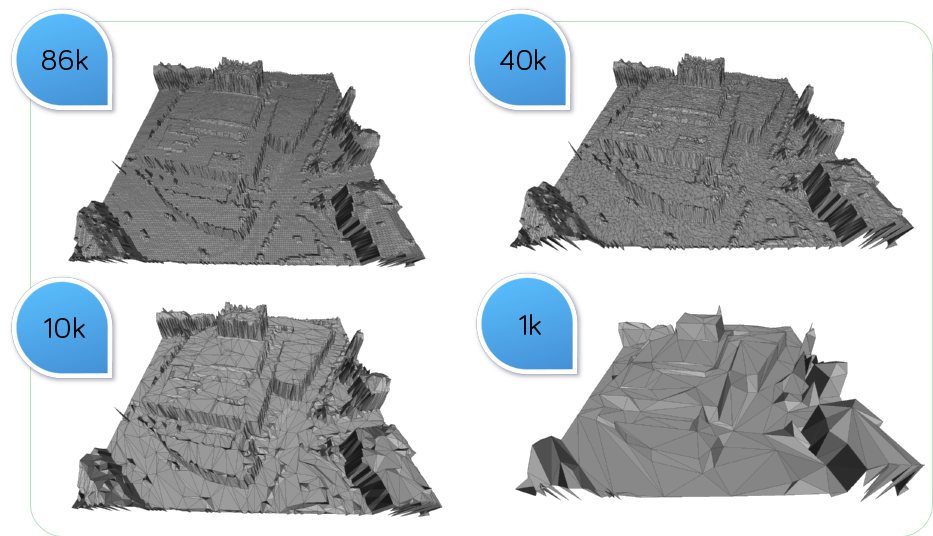
\includegraphics[width=\textwidth]{resultats.png}
   \caption{Différents seuils de réduction}
   \label{resultat}
\end{figure}

La question posée par la figure \ref{resultat} est la suivante : comment déterminer le nombre d'arêtes limite ? Dans notre exemple, on peut s'apercevoir (de manière empirique et visuelle) que la limite se situe entre 10000 et 1000 arrêtes, pour un modèle original à 86000 arêtes.

Il faudrait alors introduire, avec plus de temps, un indicateur basé sur le rapport nombre de triangles / erreur de modélisation.

On peut également obtenir des résultats similaires avec d'autres nuages de points, comme le montrent les figures \ref{b5}  \ref{b8} et \ref{b9}.

\begin{figure}[H]
  \centering
   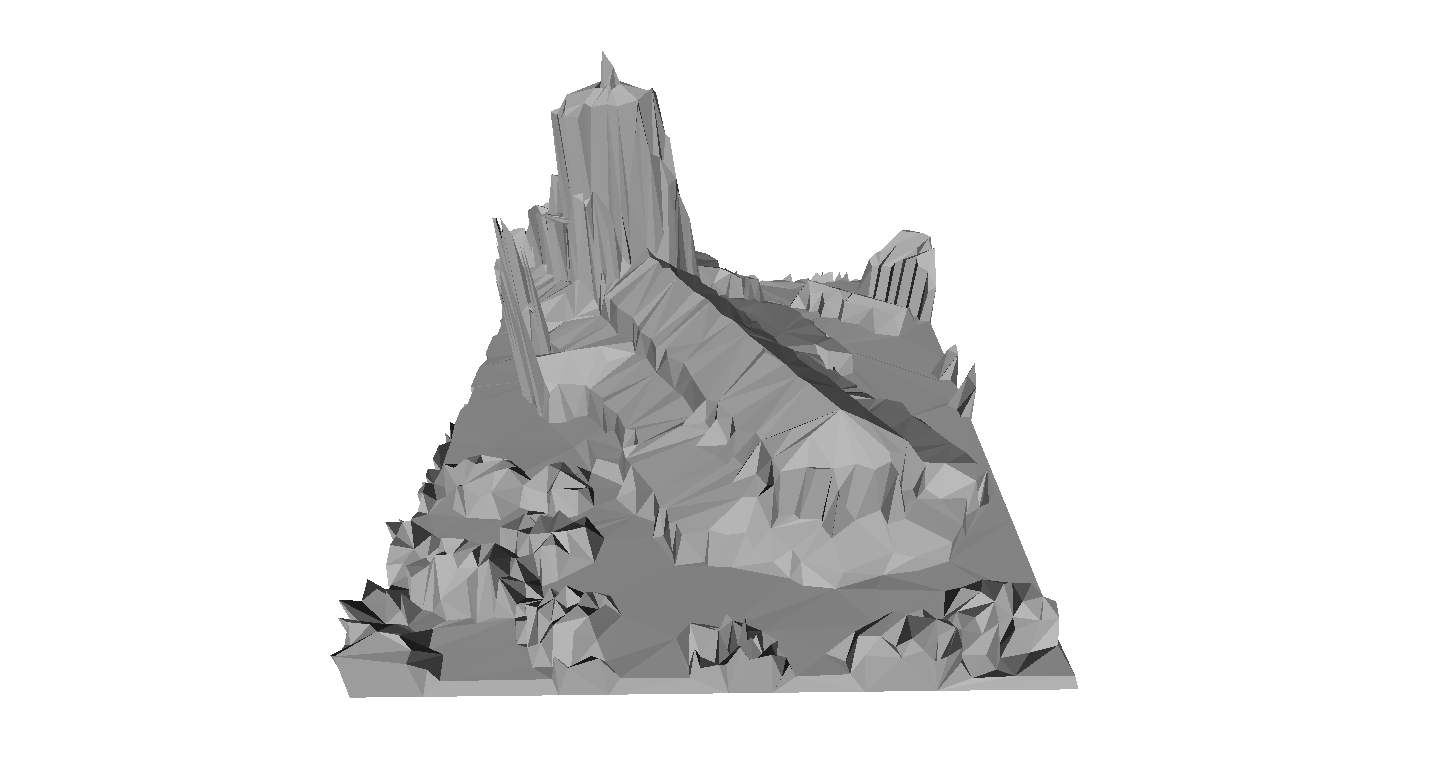
\includegraphics[width=10cm]{b5-4000.png}
   \caption{Modèle B5 avec 4000 arêtes}
   \label{b5}
\end{figure}
\begin{figure}[H]
  \centering
   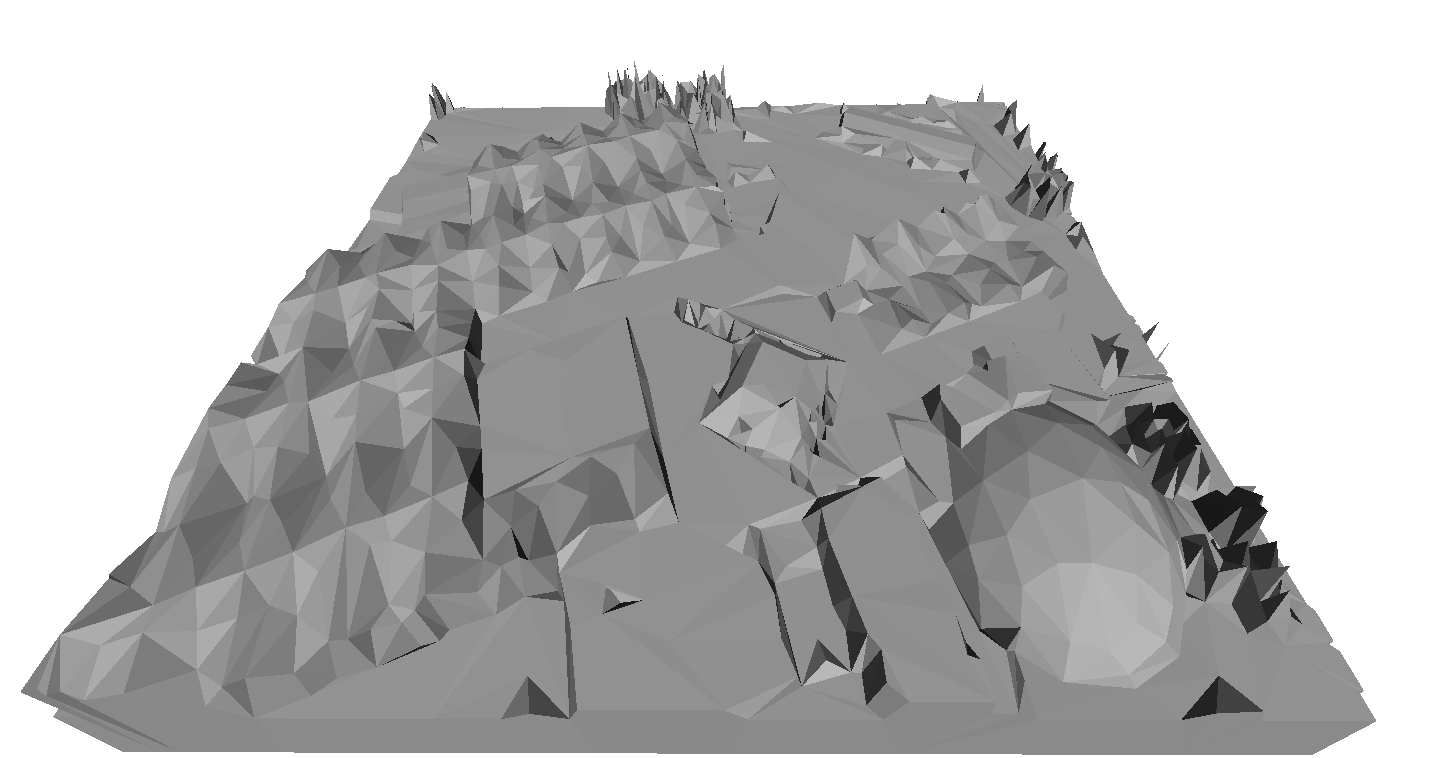
\includegraphics[width=10cm]{b8-4000.png}
   \caption{Modèle B8 avec 4000 arêtes}
   \label{b8}
\end{figure}
\begin{figure}[H]
  \centering
   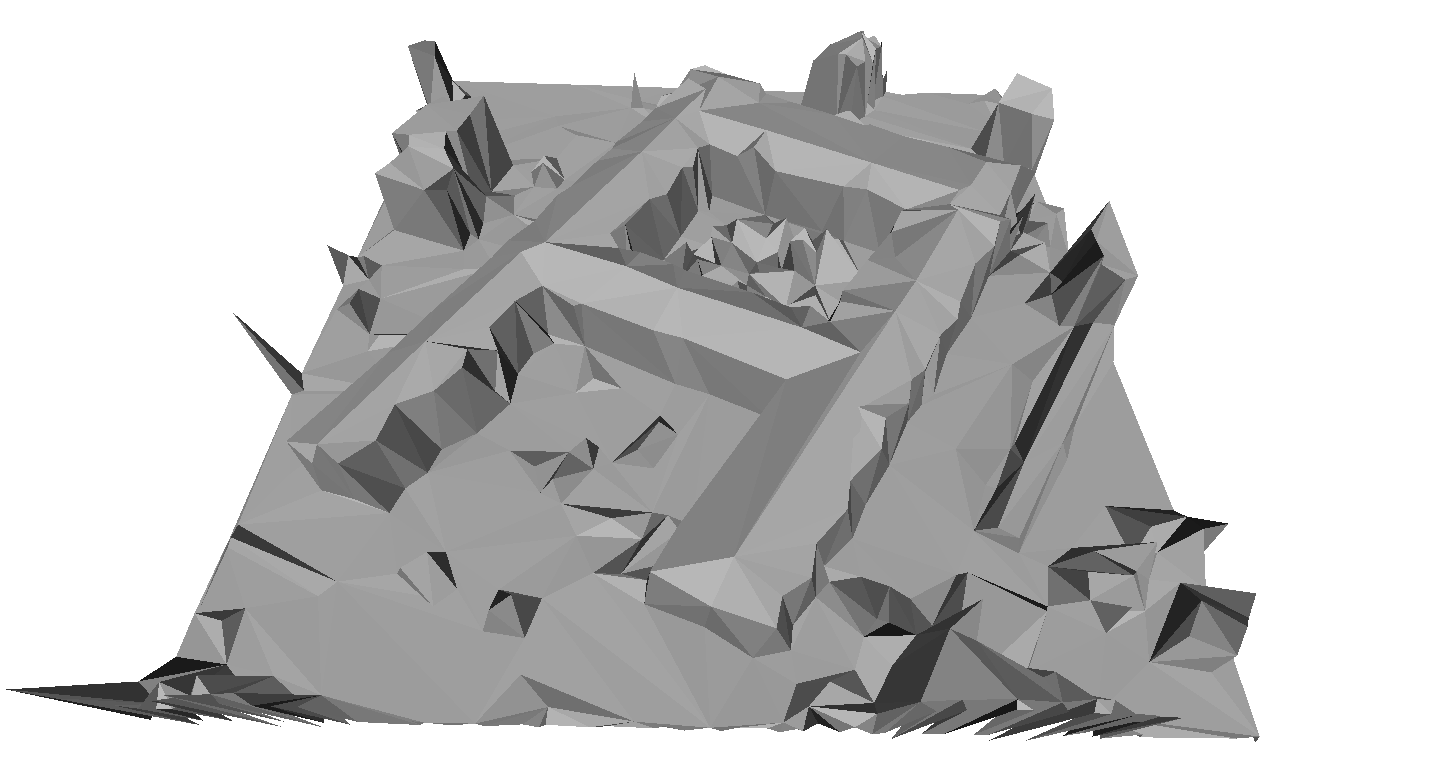
\includegraphics[width=10cm]{b9-2000.png}
   \caption{Modèle B9 avec 2000 arêtes}
   \label{b9}
\end{figure}


\subsection{Performances}
Nous pouvons également constater sans surprise que :
\begin{itemize}
 \item diminuer le nombre limite d'arêtes demande plus de temps (il faut passer plus de temps à simplifier le maillage)
 \item utiliser une grille deux fois plus dense demande beaucoup plus de temps (il y a quatre fois plus de noeud, donc six fois plus d'arêtes)
 \item le nombre initial de points dans le maillage n'est pas très significatif par rapport aux autres facteurs
\end{itemize}

\begin{center}
\begin{xtabular}[]{llll}
Points dans le nuage & Taille de la grille & Nombre cible d'arêtes & Temps \\
86021 & 170*170 & 10000 & 16s\\
86021 & 170*170 & 40000 & 7.9s\\
58499 & 120*120 & 10000 & 6.4s\\
58499 & 240*240 & 10000 & 38s\\
22300 & 149*149 & 10000 & 13s
\end{xtabular}
\end{center}
